% %%%%%%%%%%%%%%%%%%%%%%%%%%%%%%%%%%%%%%%%%%%%%%%%%%%%%%%%%%%%%%%%%%%%%%%%%%%%%
% %%%%%%%%%%%%%%%%%%%%%%%%%%%%%%%%%%%%%%%% Survey of the Near-Earth Environment
% %%%%%%%%%%%%%%%%%%%%%%%%%%%%%%%%%%%%%%%%%%%%%%%%%%%%%%%%%%%%%%%%%%%%%%%%%%%%%

\chapter{The Near-Earth Environment}
\label{ch_intro}

\todo{So far, this chapter is just a tentative outline. }

%There are a lot of interrelated things going on, so it's hard to describe Earth's environment one step at a time. Look at Scott's thesis -- he did this well, right? 

%Heliosphere, Magnetosphere, Ionosphere, Atmosphere?

%Current systems, convective systems, density profiles? 

%\begin{figure}
%  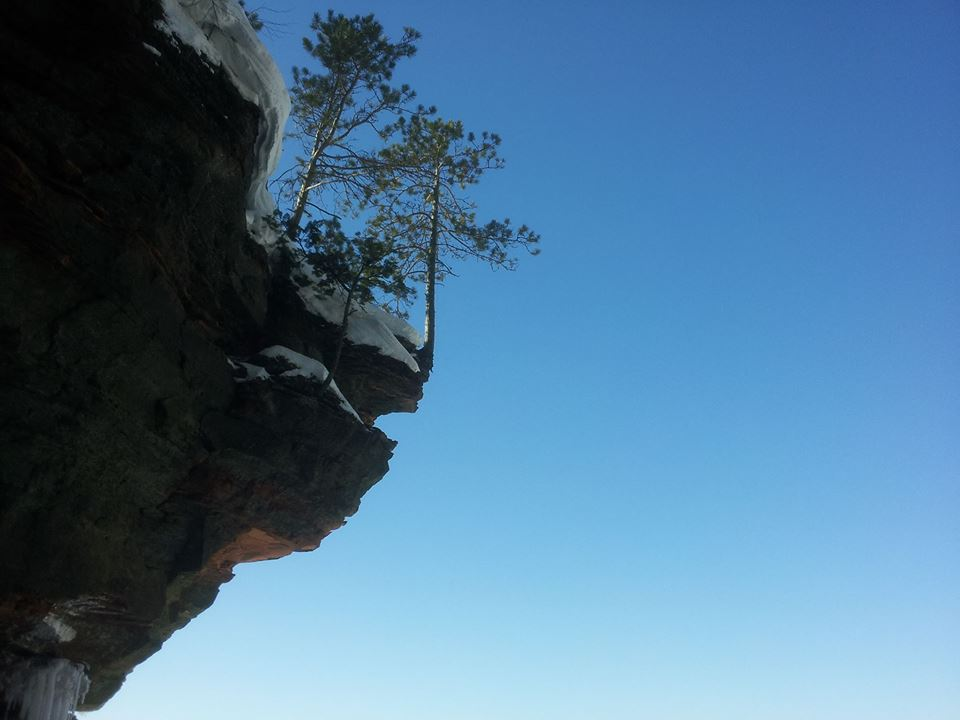
\includegraphics[width=5.75in, height=2in]{figures/image.jpg}
%  \caption{Lorem ipsum dolor sit amet, consectetur adipiscing elit, sed do eiusmod tempor incididunt ut labore et dolore magna aliqua.}
%  \label{fig_test}
%\end{figure}

It's all about energy transfer! Sun generates energy through nuclear reactions. Some of this energy is transported in the solar wind, which drives behavior in the near-Earth environment. 

%Typical solar wind density is $\sim$ \SI{5}{/\cm\cubed}. Typical solar wind velocity at Earth is \SIrange{e2}{e3}{\km/\s}. Typical solar wind particle energy is \SIrange{1}{10}{\kilo\eV}. Density can vary by $\sim$3 orders of magnitude, and velocity by one, during times of high solar activity. CMEs can also mess with the north/south component of the interplanetary magnetic field. 

At Earth's orbit, the solar magnetic field makes more-or-less a \SI{45}{\degree} angle with the \X axis. 
\footnote{Uppercase \X, \Y, and \Z are used to indicate GSE coordinates: \X points from the Earth to the Sun; \Y is perpendicular to \X in the Sun's ecliptic plane, pointing duskwards; \Z points north, out of the ecliptic plane. In later chapters, lowercase \x, \y, and \z are used to define a more-or-less analogous corodinate system with respect to Earth. }

% Solar wind is what deforms Earth's magnetic field to form the magnetosphere. 

% Transient solar wind phenomena, such as coronal mass ejections, are also known to be related to geomagnetic disturbances at Earth. Jesse cites here: 

% R. L. McPherron. Physical processes producing magnetospheric substorms and mangetic storms. In J. A. Jacobs, editor, Geomagnetism, volume 4, chapter 7. Academic Press, 1991.

% G. Rostoker. Substorms. In Handbook of the Solar-Terrestrial Environment, chapter 15. Springer-Verlag, 2007.

% This might just be worth tracking down... Jesse cites several chapters: 

% M. Shulz. Magnetospheres. In Handbook of the Solar-Terrestrial Environment, chapter 7. Springer-Verlag, 2007.

% papers mentioned during Yan's talk. mostly about alfven acceleration and nonlinear effects. 
% Vasyliunas 1970, 1984
% Hasegawa 1976
% Goertz 1991
% Stasiewicz et al 2000
% Haerendel 2008
% Song & Lysak 1994, 1999, 2000, 2001, 2006, 2011, 2012
% Inverted V?
% Double layers? 
% Charge holes? 

% =============================================================================
% =============================================================================
% =============================================================================
\section{The Outer Magnetosphere}

The outer magnetosphere is a region where the field lines are closed, but significantly deformed by the solar wind. 

\subsection{The Magnetopause}

\subsection{The Magnetotail}

\subsection{Cusp Regions}

\todo{The cusp regions might not even need to be mentioned... they're not specifically important here. }

% =============================================================================
% =============================================================================
% =============================================================================
\section{The Inner Magnetosphere}

In the inner magnetosphere, field lines are closed, and are approximately dipolar. 

\subsection{The Plasmasphere}

\subsection{Ring Currents}

\subsection{The Radiation Belts}

% =============================================================================
% =============================================================================
% =============================================================================
\section{The Ionosphere}

The ionosphere is immediately above Earth's neutral atmosphere. 

%\todo{At present, ionospheric conductivity profiles and the \Alfven speed aren't really illustrated until \cref{sec_ionos}. That's pretty awkward, since \cref{ch_math} makes extensive use of those quantities in a bunch of dispersion relations. They should be introduced before they're used! }

\subsection{Field-Aligned Currents}

\subsection{Pedersen and Hall Currents}

\subsection{Ionospheric Stratification}

% =============================================================================
% =============================================================================
% =============================================================================
\section{Geomagnetic Disturbances}

\subsection{Storms}

\subsection{Substorms}






